\chapter{Parallelisation of the Analytical Forces Induced by Dislocations on Surface Elements}
\label{c:para_f_dln_se}
	%
	\section{Parallelisation on Graphics Processing Units}
	Efficient parallelisation requires \kwd{cma}, which means we have to be extremely careful when mapping CPU memory to device memory. The fact that threads work ``simultaneously'' means that in order to obtain good performance, the data which is to be ``simultaneously'' loaded into each thread must be contiguous. This maximises cache memory use and therefore reduces slow memory fetch operations to global or shared memory.
	
	The parallelisation was done only over the \kwdp{se} in order to avoid the undesirable and inefficient GPU branching that would occur under other schemes.
	
	The most natural form of parallelisation is to have blocks of $ 4n $ threads where $ n \leq 8 \in \mathbb{N}$. This also fits nicely into the 32 thread per warp paradigm.
	%
	\subsection{Data Mapping}
		%
		\begin{figure}
			\centering
			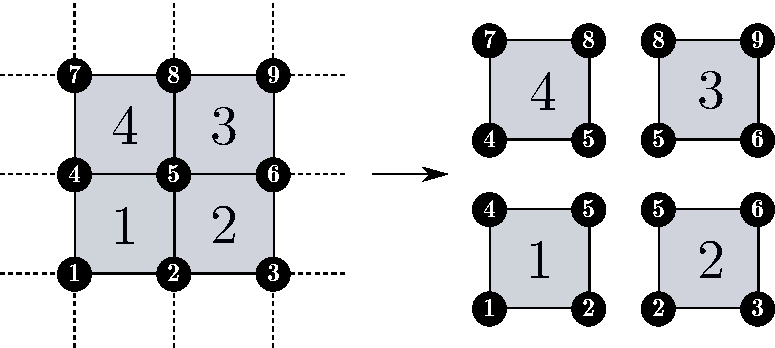
\includegraphics[width=\linewidth]{lrse_thread_map.pdf}
			\caption[Linear rectangular surface element mapping.]{Each linear rectangular \kwd{se} is mapped to one thread.}
			\label{f:lrse_map}
		\end{figure}
		%
		\subsubsection{Elements: Host $ \mapsto $ Device}
			%
			\begin{algorithm}
				\caption{Elements in host $ \mapsto $ device.}
				\label{a:ehd}
				\begin{algorithmic}[1]
					\Function{element\_host\_device\_map}{\hvar{\vec{X}[N][3\times E]}}
						\State{\Comment{Input, temporary, and output indices set to zero.}}
						\State{$ i,\, j,\, k \gets 0 $}
						\State{\Comment{\dvar{\vec{X}} accomodates all 3 coordinates of all $ N $ nodes in all $ E $ elements.}}
						\State{$ \dvar{\vec{X}} \gets $ malloc($ 3\times E\times N $)}
						\For{$(n = 0;\, n < N;\, n++)$} \Comment{Loop over nodes in element.}
							\State{\Comment{Set output index to point at the $ n\textsuperscript{th} $ node of the first coordinate of the first element.}}
							\State{$ k \gets j $}
							\For{$ (c = 0;\, c < 3;\, c++) $} \Comment{Loop over coordinates.}
								\State{\Comment{Set input index to point at the $ c\textsuperscript{th} $ coordinate of the first element of the $ n\textsuperscript{th} $ node.}}
								\State{$ i \gets c $}
								\For{$ (e = 0;\, e < E;\, e++) $} \Comment{Loop over elements.}
									\State{$ \dvar{\vec{X}[k + e]} \gets \hvar{\vec{X}[n][i]} $}
									\State{\Comment{Advance output index to point at the $ n\textsuperscript{th} $ node of the $ c\textsuperscript{th} $ coordinate of the first element.}}
									\State{$ i \gets i + 3 $}
								\EndFor
								\State{\Comment{Advance output index to point at the $ n\textsuperscript{th} $ node of the $ c\textsuperscript{th} $ coordinate of the first element.}}
								\State{$ k \gets k + E \times N $}
							\EndFor
							\State{\Comment{Advance temporary index to point at the $ (n+1)\textsuperscript{th} $ node of the first coordinate of the first element.}}
							\State{$ j \gets j + E $}
						\EndFor
						\State{\Return{\dvar{\vec{X}}}}
					\EndFunction
				\end{algorithmic}
			\end{algorithm}
		\subsubsection{Elements: Device $ \mapsto $ Thread}
			\begin{algorithm}
				\caption{Elements in device $ \mapsto $ thread.}
				\label{a:edt}
				\begin{algorithmic}[1]
						\GPUFunction[element\_device\_thread\_map]{\dvar{\vec{X}[3\times E\times N]}, \tvar{\vec{X}[N][3]}}
						\State{\Comment{Thread, input indices.}}
						\State{$ \rvar{idx},\, i \gets \rvar{threadIdx}.x + \rvar{blockIdx}.x\times \rvar{blockDim}.x $}
						\For{$ (c = 0;\, c < 3;\, c++) $}\Comment{Loop over elements.}
							\For{$ (n = 0;\, n < N;\, n++) $}\Comment{Loop over nodes in element.}
								\State{$ \tvar{\vec{X}[n][c]} \gets \dvar{\vec{X}[i + n\times E]}$}
							\EndFor
							\State{$ i \gets i + E\times N $}
							\Comment{Advance input index to the $(n+1)\textsuperscript{th}$ node of element $i$.}
						\EndFor
						\State{\Return{\tvar{\vec{X}[n][c]}}}
					\EndGPUFunction
				\end{algorithmic}    	
			\end{algorithm}
		\subsubsection{Force: Thread $ \xmapsto{+} $ Device}
			\begin{algorithm}
				\caption{Force in thread $ \xmapsto{+} $ device.}
				\begin{algorithmic}[1]
						\GPUFunction[add\_force\_thread\_device]{\tvar{\vec{F_{n}}[N][3]}, \tvar{\vec{F_{e}}[3]}, \dvar{\vec{F_{n}}[3\times E\times N]},\newline{}\dvar{\vec{F_{e}}[3\times E]}, \rvar{idx}}
						\State{\Comment{Nodal force.}}
						\State{\Comment{Set output index to whatever parallelisation index is given to the function. In this case the same index we use for the main parallelisation.}}
						\State{$ i \gets \rvar{idx} $}
						\For{$ (n = 0;\, n < N;\, n++) $} \Comment{Loop over nodes.}
							\For{$ (c = 0;\, c < 3;\, c++) $} \Comment{Loop over coordinates.}
								\State{\Comment{Ensure nodal forces are correctly added and mapped from local thread memory to global device memory.}}
								\State{atomicAdd(\dvar{\vec{F_{n}}[i + c\times E\times N]}, \tvar{\vec{F_{n}}[n][c]})}
							\EndFor
							\State{\Comment{Displace output index to point at the first coordinate of the $ (n+1)\textsuperscript{th} $ node of the \rvar{idx}\textsuperscript{th} \kwd{se}.}}
							\State{$ i \gets i + E $}
						\EndFor
						\State{\Comment{Total force.}}	
						\State{$ i \gets \rvar{idx} $} \Comment{Reset output index.}
						\For{$ (c = 0;\, c < 3;\, c++) $} \Comment{Loop over coordinates.}
							\State{atomicAdd(\dvar{\vec{F_{e}}[i]}, \tvar{\vec{F_{e}}[c]})}
							\State{\Comment{Advance the output index to point at the $ (i+1)\textsuperscript{th} $ coordinate of the $ \rvar{idx}\textsuperscript{th} $ \kwd{se}.}}
							\State{$ i \gets i + E $}
						\EndFor
						\State{\Return{\dvar{\vec{F_{n}}}, \dvar{\vec{F_{e}}}}}
					\EndGPUFunction
				\end{algorithmic}
			\end{algorithm}
		\subsubsection{Force (Parallelise over Dislocations): Thread $ \xmapsto{+} $ Device}
			\begin{algorithm}
				\caption{Force (parallelise over dislocations) in thread $ \xmapsto{+} $ device.}
				\begin{algorithmic}[1]
					\GPUFunction[dln\_add\_force\_thread\_device]{\tvar{\vec{F_{n}}[N][3]}, \tvar{\vec{F_{e}}[3]},\newline{}\dvar{\vec{F_{n}}[3\times E\times N]}, \dvar{\vec{F_{e}}[3\times E]}, $ k $}
						\State{\Comment{Nodal force.}}
						\State{\Comment{Set output index to correspond to whatever \kwd{se} we're on. By parallelising over dislocation lines, we must loop through \kwdp{se} in the main code, this is the value of $ k $ we provide. Multiply by 3 and $ N $ because each \kwd{se} has 3 coordinates and $ N $ nodes.}}
						\State{$ i \gets 3\times N\times k $}
						\State{$ j \gets 0 $} \Comment{Auxiliary index.}
						\For{$ (n = 0;\, n < N;\, n++) $} \Comment{Loop over nodes.}
							\For{$ (c = 0;\, c < 3;\, c++) $} \Comment{Loop over coordinates.}
								\State{\Comment{Ensure nodal forces are correctly added and mapped from local thread memory to global device memory.}}
								\State{atomicAdd(\dvar{\vec{F_{n}}[i + j + c]}, \tvar{\vec{F_{n}}[n][c]})}
							\EndFor
							\State{\Comment{Displace auxiliary index to point at the first coordinate of the $ (n+1)\textsuperscript{th} $ node of the $ k \textsuperscript{th}$ \kwd{se}.}}
							\State{$ j \gets j + 3 $}
						\EndFor
						\State{\Comment{Total force.}}
						\State{\Comment{Set auxiliary index to point at the first coordinate of the $ k\textsuperscript{th} $ \kwd{se}.}}
						\State{$ j \gets 3\times k $}
						\For{$ (c = 0;\, c < 3;\, c++) $} \Comment{Loop over coordinates.}
							\State{atomicAdd(\dvar{\vec{F_{e}}[j+c]}, \tvar{\vec{F_{e}}[c]})}
						\EndFor
						\State{\Return{\dvar{\vec{F_{n}}}, \dvar{\vec{F_{e}}}}}
					\EndGPUFunction
				\end{algorithmic}
			\end{algorithm}
		\subsubsection{Nodal Force: Device $ \mapsto $ Host}
			\begin{algorithm}
				\caption{Nodal force in device $ \mapsto $ host.}
				\begin{algorithmic}[1]
					\Function{fx\_device\_host\_map}{\dvar{\vec{F_{n}}[3\times E\times N]}, \hvar{\vec{F_{n}}[N][3\times E]}}
						\State{$ i,~j \gets 0 $} \Comment{Set input and output indices to zero.}
						\For{$ n = 0;\, n < N;\, n++ $} \Comment{Loop over nodes.}
							\State{$ j \gets 0 $} \Comment{Reset output index to point at the first element.}
							\For{$ e = 0;\, e < E;\, e++ $} \Comment{Loop over elements.}
								\For{$ c = 0;\, c < 3;\, c++ $} \Comment{Loop over coordinates.}
									\State{$ \hvar{\vec{F_{n}}[n][j + c]} = \dvar{\vec{F_{n}}[i + e + c\times E\times N]} $}
								\EndFor
								\State{\Comment{Advance output index to point at the first coordinate of the $ (e+1)\textsuperscript{th} $ element.}}
								\State{$ j \gets j + 3 $}
							\EndFor
							\State{\Comment{Advance input index to point at the first coordinate of the $ (n+1)\textsuperscript{th} $ node of the first element.}}
							\State{$ i \gets i + E $}
						\EndFor
						\State{\Return{\hvar{\vec{F_{n}}}}}
					\EndFunction
				\end{algorithmic}
			\end{algorithm}
		\subsubsection{Total Force: Device $ \mapsto $ Host}
			\begin{algorithm}
				\caption{Total force in device $ \mapsto $ host.}
				\begin{algorithmic}[1]
					\Function{ftot\_device\_host\_map}{\dvar{\vec{F_{e}}[3\times E]}, \hvar{\vec{F_{e}}[3\times E]}}
						\State{$ i \gets 0 $} \Comment{Set output index to zero.}
						\For{$ e = 0;\, e < E;\, e++ $} \Comment{Loop over elements.}
							\For{$ c = 0;\, c < 3;\, c++ $} \Comment{Loop over coordinates.}
								\State{$ \hvar{\vec{F_{e}}[i + c]} = \dvar{\vec{F_{e}}[e + c\times E]} $}
							\EndFor
							\State{\Comment{Advance the output index to point at the first coordinate of the $ (e+1)\textsuperscript{th} $ surface element.}}
							\State{$ i \gets i + 3 $}
						\EndFor
						\State{\Return{\hvar{\vec{F_{e}}}}}
					\EndFunction
				\end{algorithmic}
			\end{algorithm}
	\begin{subequations}\label{e:fcne}
		\begin{align}
			\vec{X}_{en}			&\coloneqq	\left[x_{en},\, y_{en},\, z_{en}\right]\\
			\vec{X}_{(1\to E)n}		&\mapsto 	\vec{X}_{n} \nn
			\vec{X}_{n}				&\coloneqq	\left[x_{1n},\, y_{1n},\, z_{1n},\ldots,x_{En},\, y_{En},\, z_{En}\right]\label{se:xn_arr}\\
			\vec{X}_{1\to N}		&\mapsto	\vec{X}^{\textrm{SE}}\nn
			\vec{X}^{\textrm{SE}}	&\coloneqq 
			\begin{aligned}
				&\left[x_{11},\, \ldots,\, x_{E1},\, x_{12},\, \ldots,\, x_{E2},\, \ldots,\, x_{1N},\, \ldots,\, x_{EN}, \right.\\
				&\left.\,y_{11},\, \ldots,\, y_{E1},\, y_{12},\, \ldots,\, y_{E2},\, \ldots,\, y_{1N},\, \ldots,\, y_{EN}, \right.\\
				&\left.\,z_{11},\, \ldots,\, z_{E1},\, z_{12},\, \ldots,\, z_{E2},\, \ldots,\, z_{1N},\, \ldots,\, z_{EN}  \right]
			\end{aligned}
		\end{align}
	\end{subequations}
	where $ e\equiv $~\kwd{se} label, $ n \equiv $~node label, $ E \equiv $~number of \kwdp{se} in the scope. $ N \equiv $~number of nodes in a \kwd{se}.
	
	Data-mapping according to \cref{a:fcne} and relabelling the nodes so they go from $ 0 \to N-1 $, the data from \cref{f:lrse_map} would be arranged in \kwd{devmem} like \cref{e:fcne_eg},
	\begin{align}\label{e:fcne_eg}
		\vec{X}^{\textrm{SE}} &= \begin{aligned}
			\left[\underbrace{h_{x},\, i_{x},\, f_{x},\, g_{x}}_{\mathbf{x_{0}}},\, 
			\underbrace{a_{x},\, b_{x},\, i_{x},\, h_{x}}_{\mathbf{x_{1}}},\, 
			\right.&\underbrace{i_{x},\, d_{x},\, e_{x},\, f_{x}}_{\mathbf{x_{2}}},\, 
			\underbrace{b_{x},\, c_{x},\, d_{x},\, i_{x}}_{\mathbf{x_{3}}},\\
			\ldots~y&\textrm{-coord}~\ldots,\\
			\ldots~z&\textrm{-coord}~\ldots]
		\end{aligned}
	\end{align}
	%
	
	In the GPU, each thread will cater to one \kwd{se} at a time. This means that each thread will have to extract the relevant data from the 1D array with length $ 3\times E\times N $ into four 1D arrays of length $ 3 $. The purpose of CNE mapping is to provide the \kwd{wrp} with \kwd{cma}. This is achieved via \cref{a:bcne}.
	
	
	Since \cref{a:bcne} is performed in a CUDA GPU, threads in a single block execute sequentially from,
	\begin{align}
		\rvar{threadIdx}.x &= 0 \to \rvar{threadIdx}.x = \rvar{blockDim}.x - 1\,,
	\end{align}
	while threads in different blocks execute in parallel. \Kwd{cma} is ensured by having each block load a cache line whose entries are contiguously accessed by the threads in the block. Using the same notation as \cref{a:fcne}, full cache line utilisation (optimal cache use) is achieved if cache lines can accomodate $ l $ entries given by \cref{e:opt_cache_len_bcne},
	\begin{align}
		\label{e:opt_cache_len_bcne}
		l =
		\begin{cases}
			a \times N \times E &,\, a > 0 \in \mathbb{N}\\
			&\textrm{or}\\
			\dfrac{1}{2^{a}} \times N \times E &,\, a \geq 0 \in \mathbb{N},\, N \times E \equiv 0\; (\bmod\; 2^{a})\,.
		\end{cases}
	\end{align}
	\Cref{f:fcne_eg} shows an example of \cref{a:bcne} up to the $ y $-coordinate.
	\begin{figure}
		\centering
		\includegraphics[width=\linewidth]{node_bmap.pdf}
		\caption[Example of the backward coodinate-node-element-map.]{Minimum working complete example of the backward coodinate-node-element-map. The explicit calculations of global indices correspond to subsituting the values for ``idx'' and ``idxi'' as in \cref{a:bcne}. $\vec{X_{a}^{b}}$ denotes a 1D array of length three containing the $ xyz $-coordinates of node $ a $ of element $ b $. Each thread concerns itself with only one element at a time. The dash-dot and dashed boxes represent cache lines for a thread block, the dotted line represents a memory fetch, and the dashed lines in $ \vec{X^{E}} $ represent steps of $ E $ entries (the start of the data for the next node of the element type we're dealing with). The memory operations are not shown twice to minimuse redundancy.}
		\label{f:fcne_eg}
	\end{figure}
	% Start: Code for generating figure e:opt_cache_len_bcne
	%\begin{align}%\label{f:fcne_eg}
	%	\vec{X}^{\textrm{SE}} &= 
	%							\begin{aligned}
	%								\left[\overbrace{h_{x},\, i_{x},\, f_{x},\, g_{x}}^{\mathbf{x_{3}}},\, 
	%								\overbrace{a_{x},\, b_{x},\, i_{x},\, h_{x}}^{\mathbf{x_{4}}},\, 
	%								\right.&\overbrace{i_{x},\, d_{x},\, e_{x},\, f_{x}}^{\mathbf{x_{5}}},\, 
	%								\overbrace{b_{x},\, c_{x},\, d_{x},\, i_{x}}^{\mathbf{x_{6}}},\\
	%								\overbrace{h_{y},\, i_{y},\, f_{y},\, g_{y}}^{\mathbf{x_{3}}},\, 
	%								\overbrace{a_{y},\, b_{y},\, i_{y},\, h_{y}}^{\mathbf{x_{4}}},\, 
	%								&\overbrace{i_{y},\, d_{y},\, e_{y},\, f_{y}}^{\mathbf{x_{5}}},\, 
	%								\overbrace{b_{y},\, c_{y},\, d_{y},\, i_{y}}^{\mathbf{x_{6}}},\\
	%								\overbrace{h_{z},\, i_{z},\, f_{z},\, g_{z}}^{\mathbf{x_{3}}},\, 
	%								\overbrace{a_{z},\, b_{z},\, i_{z},\, h_{z}}^{\mathbf{x_{4}}},\, 
	%								&\left.\overbrace{i_{z},\, d_{z},\, e_{z},\, f_{z}}^{\mathbf{x_{5}}},\, 
	%								\overbrace{b_{z},\, c_{z},\, d_{z},\, i_{z}}^{\mathbf{x_{6}}}\right]
	%\end{align}
	%\begin{align}
	%	\textrm{Parallel execution}
	%		&\begin{cases}
	%			&\vectorsym{X_{0}^{0}}[0] \gets \vectorsym{X^{E}}[(0+0\times 2) + (0\times 4 \times 4) + (0\times 4)]\nonumber\\
	%			&\vectorsym{X_{0}^{1}}[0] \gets \vectorsym{X^{E}}[(1+0\times 2) + (0\times 4 \times 4) + (0\times 4)]\nonumber\\
	%		\end{cases}\nonumber\\
	%	\textrm{Parallel execution}
	%		&\begin{cases}
	%			&\vectorsym{X_{0}^{2}}[0] \gets \vectorsym{X^{E}}[(0+1\times 2) + (0\times 4 \times 4) + (0\times 4)]\nonumber\\
	%			&\vectorsym{X_{0}^{3}}[0] \gets \vectorsym{X^{E}}[(1+1\times 2) + (0\times 4 \times 4) + (0\times 4)]\nonumber\\
	%		\end{cases}\nonumber\\
	%	\textrm{Parallel execution}
	%		&\begin{cases}
	%			&\vectorsym{X_{2}^{0}}[0] \gets \vectorsym{X^{E}}[(0+0\times 2) + (0\times 4 \times 4) + (2\times 4)]\nonumber\\
	%			&\vectorsym{X_{2}^{1}}[0] \gets \vectorsym{X^{E}}[(1+0\times 2) + (0\times 4 \times 4) + (2\times 4)]\nonumber\\
	%		\end{cases}\nonumber\\
	%	\textrm{Parallel execution}
	%		&\begin{cases}
	%			&\vectorsym{X_{2}^{2}}[0] \gets \vectorsym{X^{E}}[(0+1\times 2) + (0\times 4 \times 4) + (2\times 4)]\nonumber\\
	%			&\vectorsym{X_{2}^{3}}[0] \gets \vectorsym{X^{E}}[(1+1\times 2) + (0\times 4 \times 4) + (2\times 4)]\nonumber\\
	%		\end{cases}\nonumber\\
	%	%					
	%	\textrm{Parallel execution}
	%		&\begin{cases}
	%			&\vectorsym{X_{0}^{0}}[1] \gets \vectorsym{X^{E}}[(0+0\times 2) + (1\times 4 \times 4) + (0\times 4)]\nonumber\\
	%			&\vectorsym{X_{0}^{1}}[1] \gets \vectorsym{X^{E}}[(1+0\times 2) + (1\times 4 \times 4) + (0\times 4)]\nonumber\\
	%		\end{cases}\nonumber\\
	%	\textrm{Parallel execution}
	%		&\begin{cases}
	%			&\vectorsym{X_{0}^{2}}[1] \gets \vectorsym{X^{E}}[(0+1\times 2) + (1\times 4 \times 4) + (0\times 4)]\nonumber\\
	%			&\vectorsym{X_{0}^{3}}[1] \gets \vectorsym{X^{E}}[(1+1\times 2) + (1\times 4 \times 4) + (0\times 4)]\nonumber\\
	%		\end{cases}\nonumber\\
	%	\textrm{Parallel execution}
	%		&\begin{cases}
	%			&\vectorsym{X_{2}^{0}}[1] \gets \vectorsym{X^{E}}[(0+0\times 2) + (1\times 4 \times 4) + (2\times 4)]\nonumber\\
	%			&\vectorsym{X_{2}^{1}}[1] \gets \vectorsym{X^{E}}[(1+0\times 2) + (1\times 4 \times 4) + (2\times 4)]\nonumber\\
	%		\end{cases}\nonumber\\
	%	\textrm{Parallel execution}
	%		&\begin{cases}
	%			&\vectorsym{X_{2}^{2}}[1] \gets \vectorsym{X^{E}}[(0+1\times 2) + (1\times 4 \times 4) + (2\times 4)]\nonumber\\
	%			&\vectorsym{X_{2}^{3}}[1] \gets \vectorsym{X^{E}}[(1+1\times 2) + (1\times 4 \times 4) + (2\times 4)]\nonumber\\
	%		\end{cases}\nonumber
	%\end{align}
	% End: Code for generating figure e:opt_cache_len_bcne
	\subsubsection{Node Coordinate Element Map}
	%
	The node-coordinate-element (NCE) data mapping in \cref{e:fnce} is carried out by \cref{a:fnce}, each thread looks after a given \kwd{se}.
	\begin{algorithm}
		\caption{NCE data mapping.}
		\label{a:fnce}
		\begin{algorithmic}
			\ForAll{n nodes $ \in $ surface element}
			\ForAll{c coordinates $ \in [x,\, y,\, z] $}
			\ForAll{e surface elements $ \in $ surface mesh section}
			\State list.append(data of the $ n\textsuperscript{th}$ node with $ c\textsuperscript{th} $ coordinate of the $ e\textsuperscript{th} $ SE)
			\EndFor
			\EndFor
			\EndFor
		\end{algorithmic}
	\end{algorithm}
	\begin{subequations}\label{e:fnce}
		\begin{align}
			\vec{X}_{en}			&\coloneqq \left[x_{en},\, y_{en},\, z_{en}\right]\\
			\vec{X}_{(1\to E)n}		&\mapsto \vec{X}_{n} \nn
			\vec{X}_{n}				&\coloneqq \left[x_{1n},\ldots,\, x_{En},\, y_{1n},\ldots,\, y_{En},\, z_{1n},\ldots,\, z_{En}\right]\\
			\vec{X}_{1\to N}		&\mapsto \vec{X}^{\textrm{SE}}\nn
			\vec{X}^{\textrm{SE}}	&\coloneqq 
			\begin{aligned}
				\left[x_{11},\ldots,\, x_{E1},\, y_{11},\right.&\ldots,\, y_{E1},\, z_{11},\ldots,\, z_{E1}\\
				,&\ldots,\\
				x_{1M},\ldots,\, x_{EN},\, y_{1N},&\left.\ldots,\, y_{EN},\, z_{1N},\ldots,\, z_{EN}\right]
			\end{aligned}
		\end{align}
	\end{subequations}
	where $ e\equiv $~surface \textbf{e}lement, $ n \equiv $~\textbf{n}ode, $ E \equiv $~total number of \kwdp{se} in scope, $ N \equiv $~total number of nodes in each \kwd{se}.
	
	Data-mapping according to \cref{a:fnce} and relabelling the nodes so they go from $ 0 \to N-1 $, the data from \cref{f:lrse_map} would be arranged in \kwd{devmem} like \cref{e:fnce_eg},
	\begin{align}\label{e:fnce_eg}
		\vec{X}^{\textrm{SE}} &= \begin{aligned}
			&\left[\underbrace{h_{x},\, i_{x},\, f_{x},\, g_{x},\, 
				h_{y},\, i_{y},\, f_{y},\, g_{y},\, 
				h_{z},\, i_{z},\, f_{z},\, g_{z}}_{\mathbf{x_{0}}}\right.,\\
			&~\ldots~\mathbf{x_{1}},\, xyz\textrm{-coords}~\ldots,\\
			&~\ldots~\mathbf{x_{2}},\, xyz\textrm{-coords}~\ldots,\\
			&~\ldots~\mathbf{x_{3}},\, xyz\textrm{-coords}~\ldots]
		\end{aligned}
	\end{align}
	%
	\subsubsection{Resolving Data Write Conflicts}
	Data write conflicts can be a problem in parallel applications where global data is changed by multiple threads within the same clock tick. This can be avoided with \kwdp{atop}.
	%
	\subsection[Parallel Dislocation Line Segments to Surface Elements]{Resolving Parallel Dislocation Line Segments to Surface Elements}
	%
	Dealing with the special case when the \kwd{dls} $ \vec{t} $ is parallel to the \kwd{se} is relatively trivial when in a serial program. By the mean value theorem, we can slightly perturb $ \vec{t} $ by rotating it by a small angle around the midpoint of $ \vec{t} $ with respect to the axis of rotation defined by $ \vec{t} \times \vec{n} $. In contrast to serial code, program branches can have a serious effect on parallel performance due to \kwd{wrpd}. Due to the complexity of the force calculation and relative rarity of the edge case, there is no branching behaviour in the parallel code until \emph{after} the calculation is performed. Where \cref{a:plse_p} is performed.
	\begin{algorithm}
		\caption{Resolving cases when $ \vec{t} \parallel \vec{n} $ on GPUs.}
		\label{a:plse_p}
		\begin{algorithmic}
			\ForAll{surface elements \emph{and} line segments}
			\State $ \ldots $
			\If{$ \vec{t}_{\textrm{thread}} \parallel \vec{n}_{\textrm{thread}} $}
			\State $ \vec{x}_{\textrm{buffer}} \gets \vec{x}_{\textrm{thread}} $
			\State $ \vec{t}_{\textrm{buffer}} \gets \vec{t}_{\textrm{thread}} $
			\Else
			\State $ \vec{F}_{\textrm{total}} += \vec{F}_{\textrm{thread}} $
			\EndIf
			\EndFor
			\State return to serial code
			\If{$ \vec{x}_{\textrm{buffer}} \neq $ empty}
			\ForAll{surface elements \emph{and} line segments}
			\State perform calculation for $ \vec{t} \parallel \vec{n} $
			\EndFor
			\EndIf
		\end{algorithmic}
	\end{algorithm}
	\subsubsection{Implementation}
	The node mapping would be the same as \cref{a:fcne}. The parallelisation would be on individual packets of a \kwd{se} with a slightly rotated \kwd{dls}, as in a single iteration of the serial code where the \kwd{dls} is rotated. The forces would be averaged with \kwdp{atop} and \mintinline{c}{__syncthreads()} before they are added to the total nodal forces.
	
	\subsection{Test Case}
	\begin{figure}
		\includegraphics[width=\linewidth]{cuda_test.pdf}
		\caption[Test case for CUDA development.]{Test case for CUDA development. Dislocation line not shown in node separation as the parallelisation happens across surface elements. Not to perspective or scale.}
		\label{f:cuda_test}
	\end{figure}
	According to \cref{a:fcne} and the node labelling scheme of \cref{f:flrs} the data mapping would look like:
	\begin{align}\label{e:cuda_test}
		\vec{X}^{\textrm{SE}} = 
		\begin{split}
			\left[\overbrace{\underbrace{1,1,0,0}_{\mathbf{x_{3}}}, \underbrace{2,2,1,1}_{\mathbf{x_{4}}},
				\underbrace{1,1,0,0}_{\mathbf{x_{5}}}, \underbrace{2,2,1,1}_{\mathbf{x_{6}}}}^{x\textrm{-coord}},\right.\\
			\overbrace{\underbrace{0,1,1,0}_{\mathbf{x_{3}}}, \underbrace{0,1,1,0}_{\mathbf{x_{4}}},
				\underbrace{1,2,2,1}_{\mathbf{x_{5}}}, \underbrace{1,2,2,1}_{\mathbf{x_{6}}}}^{y\textrm{-coord}},\\
			\left.\overbrace{\underbrace{0,0,0,0}_{\mathbf{x_{3}}}, \underbrace{0,0,0,0}_{\mathbf{x_{4}}},
				\underbrace{0,0,0,0}_{\mathbf{x_{5}}}, \underbrace{0,0,0,0}_{\mathbf{x_{6}}}}^{z\textrm{-coord}}\right]
		\end{split}
	\end{align}
	In general the number of indices in the array would be $ 3 \times e \times n $ where $ e \equiv $~number of surface elements, $ n \equiv $~number of nodes per element and 3 is the number of spatial dimensions.
	\savearabiccounter